% This must be in the first 5 lines to tell arXiv to use pdfLaTeX, which is strongly recommended.
\pdfoutput=1
% In particular, the hyperref package requires pdfLaTeX in order to break URLs across lines.

\documentclass[11pt]{article}

% Change "review" to "final" to generate the final (sometimes called camera-ready) version.
% Change to "preprint" to generate a non-anonymous version with page numbers.
\usepackage[review]{acl}

% Standard package includes
\usepackage{times}
\usepackage{latexsym}

% For proper rendering and hyphenation of words containing Latin characters (including in bib files)
\usepackage[T1]{fontenc}
% For Vietnamese characters
% \usepackage[T5]{fontenc}
% See https://www.latex-project.org/help/documentation/encguide.pdf for other character sets

% This assumes your files are encoded as UTF8
\usepackage[utf8]{inputenc}

% This is not strictly necessary, and may be commented out,
% but it will improve the layout of the manuscript,
% and will typically save some space.
\usepackage{microtype}

% This is also not strictly necessary, and may be commented out.
% However, it will improve the aesthetics of text in
% the typewriter font.
\usepackage{inconsolata}

%Including images in your LaTeX document requires adding
%additional package(s)
\usepackage{graphicx}

% If the title and author information does not fit in the area allocated, uncomment the following
%
%\setlength\titlebox{<dim>}
%
% and set <dim> to something 5cm or larger.

\title{Homework 1B}


\author{Paolo Renzi \\
  Sapienza Università di Roma\\\
  }


% Introduction
% Description of the dataset (brief)
% Architecture of your model (figures are okay) 
% Design choices of your model (why did you choose to do x instead of y?)
% Baselines implemented (brief)
% Results section (how does your model compare to the baselines?)
% Instructions to run your code (unambiguous)
% Any other information you think may be useful for us



\begin{document}
\maketitle

\section{Description of the dataset}
The dataset comprises two tasks aimed at detect-
ing hate speech. Task 1 focuses on Hate Speech
Detection, where the goal is to classify whether a
message contains hate speech or not. The training
set consists of 5,600 tweets from PolicyCorpusXL,
while the test set includes 1,400 tweets from Poli-
cyCorpusXL and 3,000 tweets from ReligiousHate.
In Task 2, termed Contextual Hate Speech Detec-
tion, both the content of tweets and their meta-
data are considered for classification. This task
includes two sub-tasks: Political Hate Speech De-
tection, which utilizes data from both development
and test sets from PolicyCorpusXL, and Religious
Hate Speech Detection, where only the test data
from ReligiousHate is provided, adapted from an
original cross-domain task.

\section{Architecture of your model}
My model is a bidirectional LSTM with a projection layer at the end.

\begin{figure}[!htb]
  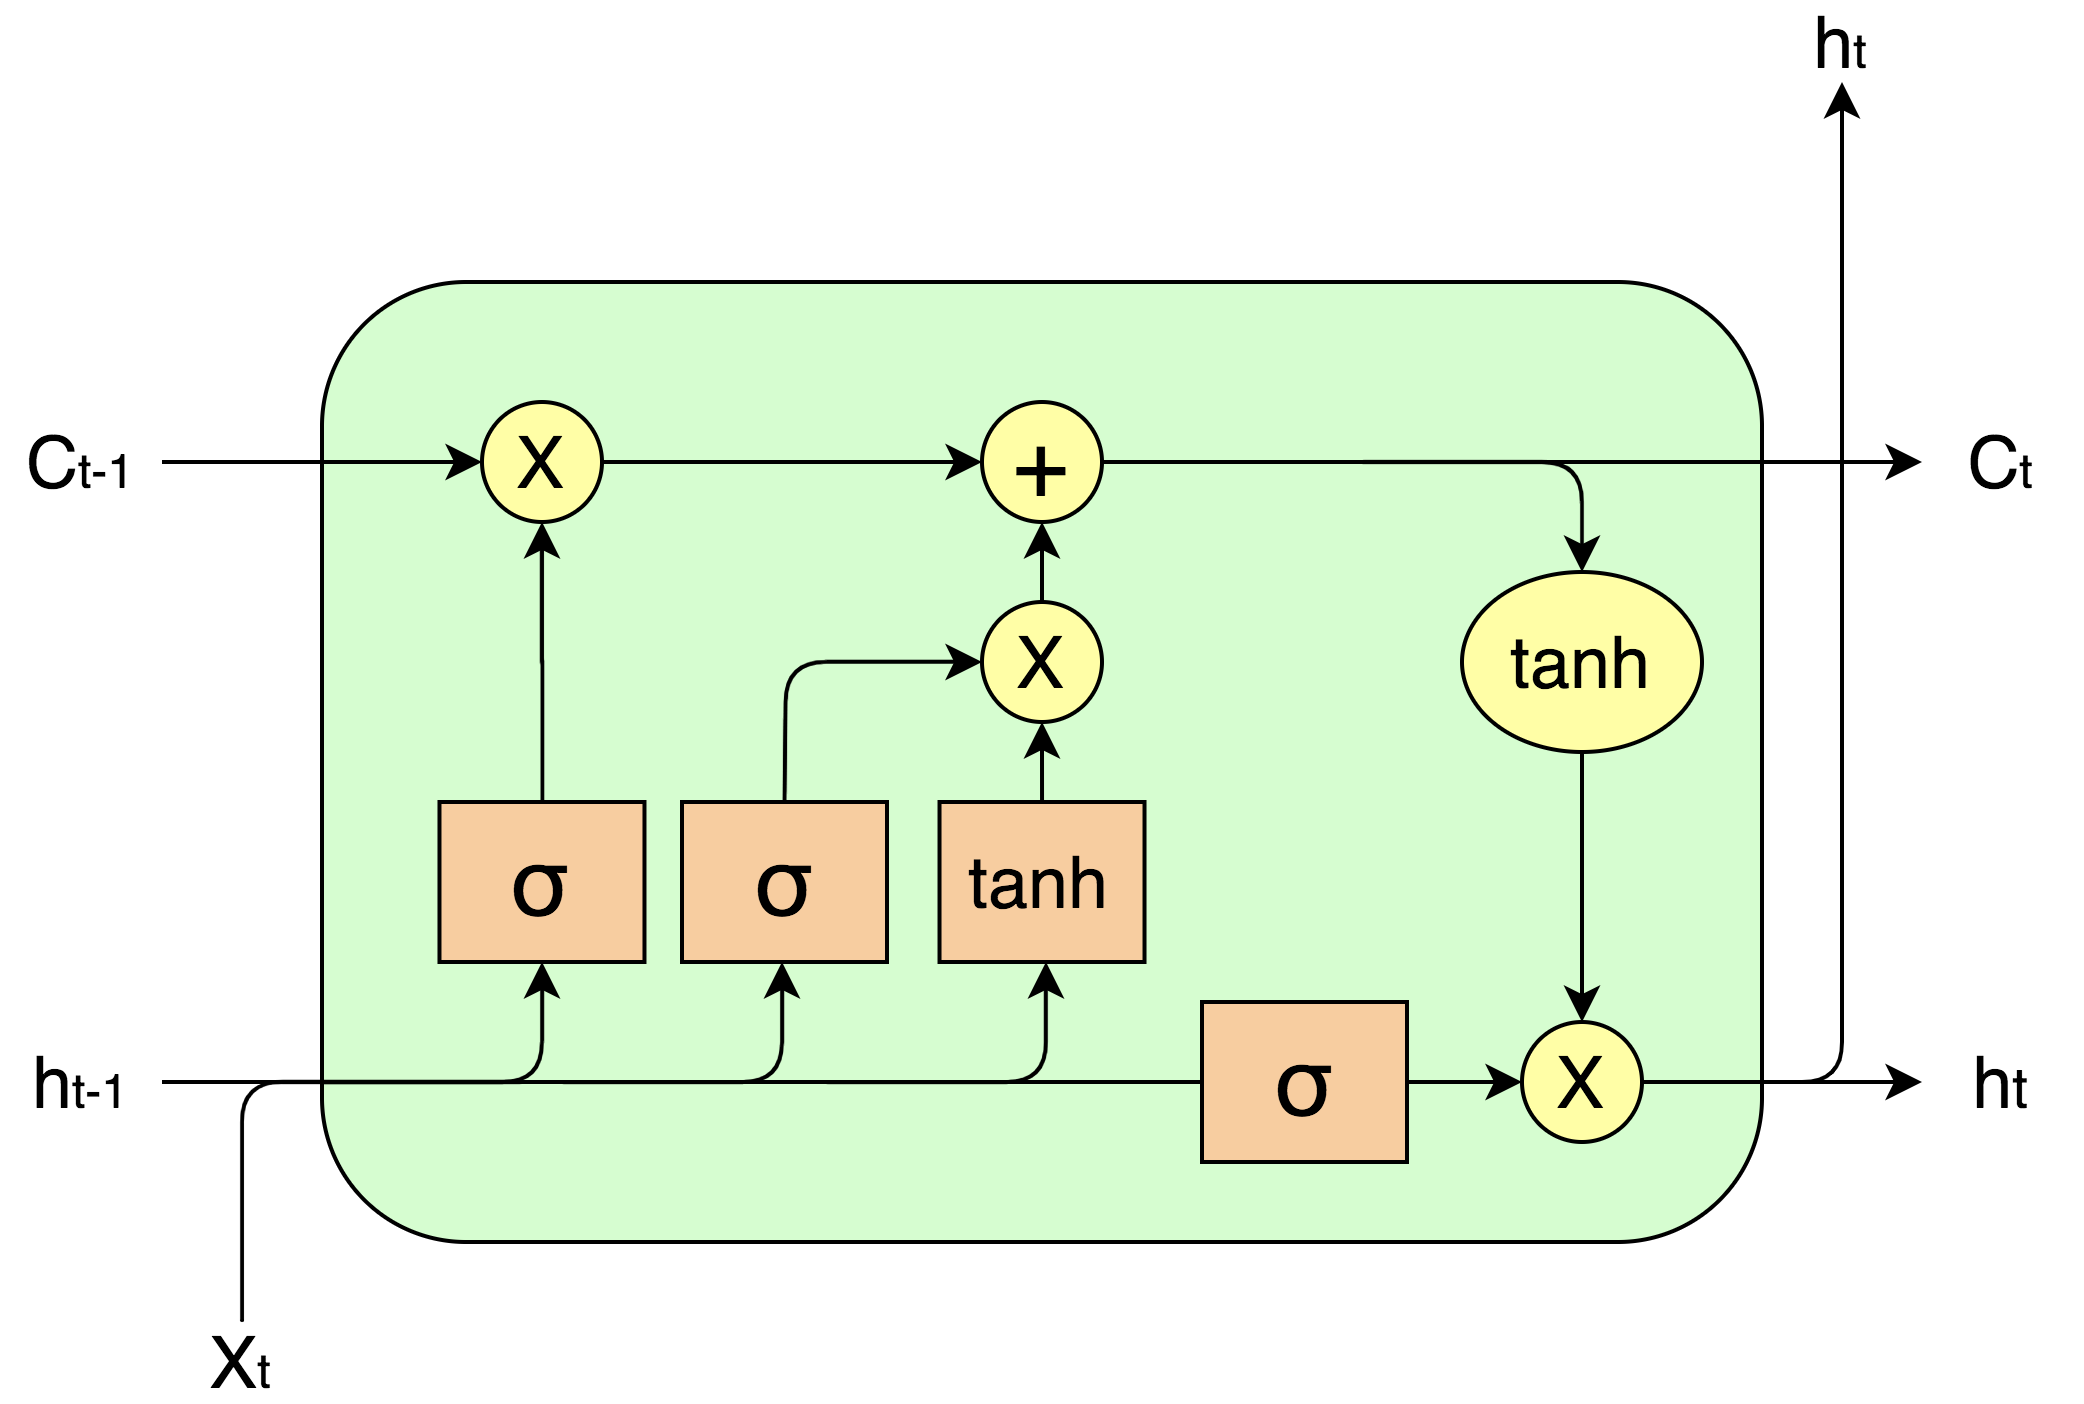
\includegraphics[width=\columnwidth]{LSTM.png}
  \label{fig:LSTM}
\end{figure}

\section{Design choices of your model}
I used a low number of layers and the hidden size because I noticed that the dataset was quite easy to calssify so it didn't need a too complex model

\section{Baselines implemented}
I implemented 2 baselines, a random one, that simply generates a random tensor of the desired dimensions and an RNN 

\section{Results section}

LSTM: 

\[Epoch: 20\] train loss = 0.6384
\[Epoch: 20\] valid loss = 0.6380, valid acc = 0.9961
Test loss 0.6359703506742205, Test accuracy: 0.9959821428571428

RNN:
\[Epoch: 20\] train loss = 0.5663
\[Epoch: 20\] valid loss = 0.5644, valid acc = 0.8583

Test loss 0.5634483064923967, Test accuracy: 0.8554315481867109

I noticed that the results vary drastically dependeding on the initialization, it can either overfit from the beginning or starting from a bad initialization 
might mean that the initial accuracy is 0.000, and that's for both the LSTM and RNN.

\section{Instructions to run your code}
To run the training you should set the folder contating
hw1b\_train.py as CWD and then run
python hw1b\_train.py
as for the evaluation you should get to the same folder and run
python hw1b\_evaluate.py

\end{document}
